\documentclass[12pt]{report}
%\usepackage{natbib}
\usepackage[
	backend=bibtex,
	style=numeric,
]{biblatex}
\addbibresource{bibliographie}


\usepackage[english]{babel}
\usepackage[utf8]{inputenc}
\usepackage[T1]{fontenc}
\usepackage[a4paper,left=3cm,right=2.5cm,top=3cm,bottom=3cm, twoside]{geometry}
\usepackage{xcolor}
\usepackage{stmaryrd}
\usepackage{amssymb}
\usepackage{amsmath}
\usepackage{libertine}
\usepackage[pdftex]{graphicx}
\usepackage{caption}
\usepackage{subcaption}
\usepackage{float}
\usepackage{multirow}
\usepackage{apalike}
\usepackage{minitoc}
\usepackage{tikz}
\usepackage{enumitem}
\usepackage{epigraph}
%\usetikzlibrary{shadows.blur}
\usepackage{lscape}
\usepackage{titletoc}
%\usepackage{lipsum}
%\usepackage{cite}
\usepackage{booktabs}
\usepackage{arydshln}
\usepackage[nonumberlist]{glossaries}
\usepackage{calc}
\usepackage{color}
\definecolor{shadecolor}{rgb}{0.92,0.92,0.92}
\usepackage{framed}
\usepackage{colortbl}
\usepackage[]{titlesec} 
\definecolor{linkColor}{HTML}{32a852}
\usepackage[colorlinks=true,citecolor=linkColor,linkcolor=black]{hyperref}
\usepackage{fancyhdr}
\usepackage{lipsum}
\usepackage{listings}
\lstset{
 columns=fixed,       
 numbers=left,                                        % 在左侧显示行号
 numberstyle=\helvetica\color{gray},                       % 设定行号格式
 frame=none,                                          % 不显示背景边框
 backgroundcolor=\color[RGB]{245,245,244},            % 设定背景颜色
 keywordstyle=\color[RGB]{40,40,255},                 % 设定关键字颜色
 numberstyle=\footnotesize\color{darkgray},           
 commentstyle=\it\color[RGB]{0,96,96},                % 设置代码注释的格式
 stringstyle=\rmfamily\slshape\color[RGB]{128,0,0},   % 设置字符串格式
 showstringspaces=false,                              % 不显示字符串中的空格
 language=python,                                        % 设置语言
}

%%%%%%%%%%%%%%%%%%%%%%%%%%%%%%%%%%%%%%%%%%%%%%%%%%%%%%%%%%%%%%%%%%%%%%%%%%
%%%%%%%%%%%%%%%%%%%%%%%%%%%%%%%%%%%%%%%%%%%%%%%%%%%%%%%%%%%%%%%%%%%%%%%%%%

\definecolor{yourcolor}{HTML}{8a0e19}%{008bb2}

\titleformat{\chapter}[display]
{\normalfont\color{yourcolor}}
{\filleft\huge\color{black}\textsc\chaptertitlename\hspace*{2mm}%
	\begin{tikzpicture}[baseline={([yshift=-.6ex]current bounding box.center)}]
	\node[fill=yourcolor,circle,text=white] {\thechapter};
	\end{tikzpicture}
}
{1ex}
{\titlerule[1.5pt]\vspace*{1.5ex}\Huge\color{black}\textsc}
[]

\titleformat{name=\chapter,numberless}[display]
{\normalfont\color{black}}
{}
{1ex}
{\vspace*{-5cm}\Huge\textsc}
[]

%command to print the acutal minitoc
\newcommand{\printmyminitoc}[1]{%
	\noindent\hspace{1cm}%
	\colorlet{chpnumbercolor}{black}%
	\begin{tikzpicture}
	\node(s){
		\begin{minipage}{.9\linewidth}%minipage trick
		\printcontents[]{}{}{}
		\end{minipage}
	};
	{
		\color{yourcolor}
		\draw(s.north west)--(s.north east) (s.south west)--(s.south east);
	}
	\end{tikzpicture}
	\vspace*{3ex}
	
	#1
	\vfill
	\pagebreak
}


\newcommand{\HRule}{\rule{\linewidth}{0.7mm}}
\newcommand{\Hrule}{\rule{\linewidth}{0.3mm}}

%%%%%%%%%%%%%%%%%%%%%%%%%%%%%%%%%%%%%%%%%%%%%%%%%%%%%%%%%%%%%%%%%%%%%%%%%%%%%
%%%%%%%%%%%%%%%%%%%%%%%%%%%%%%%%%%%%%%%%%%%%%%%%%%%%%%%%%%%%%%%%%%%%%%%%%%





\begin{document}
	
	\begin{titlepage}
		\begin{center}
			\begin{tabular}{c@{\hskip 20cm}c}
				
\includegraphics[height=2cm]{images/UniversiteParisCite_logo_horizontal_couleur_CMJN.jpg}
			\end{tabular}
		\end{center}
	
		
		\begin{center}

			Université de Paris Cité\\
			L3 MIASHS - OPTIMISATION
  
  			\vfill
  			
	 		\HRule \\[0.1cm]
	 		 { \Large \bfseries Projet 10	 }
	  		\HRule \\
		
		\end{center}
		
		\vfill
			
		\begin{center}
			Présenter par \\ \textsc{\Large Ying YE : 71803144 \\
			Hengze WANG : 71806536}\\[1cm] 
		
	
			
			\vspace{1cm}
	
			 Avril 2022
		\end{center}
		
		\vspace{1cm}
			
		
		

	\newpage
	\end{titlepage}



\pagestyle{plain}

\fancyhead{}





\setlength{\parskip}{.7em}

\titlespacing*{\section}{0pt}{.9em}{.8em}
\renewcommand{\baselinestretch}{1.1}


\fancyhead[RO]{\leftmark}
\fancyhead[LE]{\textsc{\chaptername~\thechapter}}

\begin{flushleft}
Une entreprise fabrique deux modèles de petites voitures, les modèles X et Y. Le modèle X, le plus aborable, se vend à 10 $\$$ pièce.  Quant au modèle Y, beaucoup plus sophistiqué, il se vend à 30 $\$$. Le coût de fabrication, exprimé en $\$$, est donné par la fonction suivante : 

$$c(x,y) = 5x^2 + 5y^2 - 2xy - 160x - 80y$$

où $x$ est le nombre de petites voitures du modèle $X$ et $y$ est le nombre de petites voitures du modèle $Y$. On suppose que les jouets fabriqués sonnt tous écoulés sur le marché.\end{flushleft} \\

\begin{flushleft}
\textbf{
1) Donner le profit p(x,y) de l'entreprise lorsqu'elle a venndu x jouets de modèle X et y jouets de modèle Y. La fonction p est-elle convexe / concave sur $\mathbb{R}^2_{+}$ ?}\end{flushleft}\\
\begin{flushleft}
Soit le coût de vente noté $v(x,y)$, on a que $v(x,y) = 10x + 30y$.
Donc on sait que le profit
\begin{align*}
    p(x,y) &= v(x,y) - c(x,y) \\
    &= 10x + 30y - (5x^2 + 5y^2 - 2xy - 160x - 80y)\\
    &= -5x^2 + 170x + 2xy - 5y^2 + 110y
\end{align*}
On calcule le gradient de $p(x,y)$, on a :
$$\nabla p(x,y) = \begin{pmatrix} -10x + 2y + 170 \\ -10y + 2x + 110 \end{pmatrix}$$
En suite, on calcule son matrice hessienne, on a :
$$\mathbb{H}p(x,y) = \begin{pmatrix} -10 & 2 \\ 2 & -10 \end{pmatrix} $$
on obtient que
\begin{align*}
    &Tr(\mathbb{H}p(x,y)) = -20 < 0, \\
    &det(\mathbb{H}p(x,y)) = 96 > 0 \\
    &\Rightarrow \mathbb{H}p(x,y) \prec 0
\end{align*}
Le determinant de la Hessienne vaut 96 et la trace vaut -20, ainsi, les valeurs propres sont de même signes et sont strictement négatives. La fonction $p$ est donc fortement concave, donc elle possède un unique point de maximum sur $\mathbb{R}^2_{+}$.\end{flushleft}\\ 

\begin{flushleft}
\textbf{
2) La capacité de production de l'entreprise est au total 25 jouets par jour. En supposant que l'entreprise tourne à plein régime, trouver la répartition maximale entre les modèles de type X et Y permettrant de maximiser le profit quotidien. Calculer dans ce cas le profit réalisé.}\end{flushleft}

\begin{flushleft}
L'entreprise est au total 25 jouets par jour , alors $x + y \leq 25$
Pour trouver la répartition maximale, on doit trouver les maxima de la fonction 
$$p(x,y) = -5x^2 + 170x + 2xy - 5y^2 + 110y$$ 
sous la contrainte $x + y \leq 25$.
Le gradient de la fonction $p(x,y)$ est 
$$\nabla p(x,y) = \begin{pmatrix} -10x + 2y + 170 \\ -10y + 2x + 110 \end{pmatrix}$$
La contrainte peut s'écrire $g(x,y) \leq 0$, où $g(x,y) = x + y - 25$. Le gradient de la fonction $g(x,y)$ est 
$$\nabla g(x,y) = \begin{pmatrix} 1 \\ 1 \end{pmatrix}$$
On cherche un minimum $(x^*,y^*)$ de $p$ sur l'ensemble $K = \{(x,y) : g(x,y) \leq 0 \}$. On distingue deux situations :\\
 - Le point est à l'intérieur dans $K° = \{(x,y) : g(x,y) < 0\}$ i.e. la contrainte est inactive. Alors
 $$\nabla p(x,y) = 0$$
 dont la solution est
 $$\begin{cases} 0 < x < \frac{55}{3} \\ 0 < y < \frac{20}{3} \\x + y < 25\end{cases}$$
 Donc il n'y a pas de solution.
 \\- Le point est sur le bord $\partial K = \{(x,y) : g(x,y) = 0 \}$ i.e. la contrainte est active. Dans ce cas, il existe $\lambda \in \mathbb{R}$ tel que
 $$\begin{cases} \nabla p(x,y) = \lambda \nabla g(x,y) \\ g(x,y) = 0 \end{cases}$$
 On peut réécrire cette condition sous la forme du système suivant
$$\begin{cases} -10x + 2y + 170 = \lambda \\ -10y + 2x + 110 = \lambda \\ x + y - 25  = 0\end{cases}$$
On trouve que 
$$\begin{cases} x = 20 - \frac{1}{8}\lambda \\ y = 15 - \frac{1}{8}\lambda \end{cases}$$
Maintenant, on élimine $\lambda$ en utilisant la conntrainte qui dit que 
$$0 = g(x,y) = g(20 - \frac{1}{8}\lambda , 15 - \frac{1}{8}\lambda) = 10 -\frac{1}{4}\lambda$$
Donc $\lambda = 40$. On injecte cela dans les expressions de $x,y$ trouvées au dessus pour obtenir
$$\begin{cases} x = 15 \\ y  = 10 \end{cases}$$
Observons que $p(15,10) = 2325$

 
Donc la répartition maximale entre les modèles de type X et Y permettant de maximiser le profit quotidien : 
 - Produire 15 voitures du modèle X et 10 voitures du modèle Y, dans ce cas le profit réalisé est 2325 $\$$.\end{flushleft}\\

\begin{flushleft}
\textbf{ 
3) Le conseil d'administration de l'entreprise s'interroge sur la pertinence de vouloir produire à pleine capacité. Il se demande s'il ne peut pas augmenter le profit en produisant autrement. Pouvez-vous aider le conseil d'administration?}\end{flushleft}\\
\begin{flushleft}
On cherche
$$sup_{(x,y)\in \mathbb{R}^2_{+}} p(x,y)$$
On a déjà que 
$$\nabla p(x,y) = \begin{pmatrix} -10x + 2y + 170 \\ -10y + 2x + 110 \end{pmatrix}$$
et
$$\mathbb{H}p(x,y) = \begin{pmatrix} -10 & 2 \\ 2 & -10 \end{pmatrix} $$
La fonction est donc concave, elle possède dont un unique point de maximum sur $\mathbb{R}^2_{+}$, on calcule en annulant le gradient, Donc on a :
$$\begin{cases} -10x + 2y + 170 = 0 \\ -10y + 2x + 110 = 0 \end{cases}$$
Dont l'unique solution est :
$$\begin{cases} x = 20 \\ y = 15 \end{cases}$$
Ainsi,
$$max~p = p(20,15) = 2525$$
Dans ce cas, le profit va être 2525 $\$$.\\
Donc, à notre avis, on va conseiller le conseil d'administration de l'entreprise de produire 20 voitures de modèle X et 15 voitures de modèle Y par jour pour avoir le profit maximum.\end{flushleft}\\

\begin{flushleft}
\textbf{
4) Ecrire un programme Python qui : \\
\end{flushleft}
a) affiche le graphe de la surface associé à la fonction bénéfice $p$ et ses lignes de niveau;}\\
\begin{lstlisting}
# Rajouter ici toutes les librairies necessaires 

import numpy as np
from numpy import exp, sin, cos, sqrt

import matplotlib.pyplot as plt
from mpl_toolkits import mplot3d

import scipy
from scipy import optimize as opt

from IPython.core.interactiveshell import InteractiveShell
InteractiveShell.ast_node_interactivity = "all"
\end{lstlisting}

\begin{lstlisting}
#la fonction du cout de production c
def c(x):
    return 5*x[0]**2+5*x[1]**2-2*x[0]*x[1]-160*x[0]-80*x[1]
#la fonction du chiffre d'affaires v
def v(x):
    return 10*x[0] + 30*x[1]
#la fonction du profil p
def p(x):
    return v(x)-c(x)
    
#maillage pour le graphe
x = np.linspace(0,50,100)
y = np.linspace(0,50,100)
X,Y = np.meshgrid(x,y)
Z = p([X,Y])
#trace
fig = plt.figure(figsize=(7,7))
ax = plt.axes(projection='3d')
ax.plot_surface(X,Y,Z,cmap = 'viridis')
#affichage de contours
fig = plt.figure(figsize=(7,7))
plt.contour(X,Y,Z,20)
plt.plot(20,15,'r*')
plt.colorbar()
\end{lstlisting}

\begin{figure}[h!]
    \caption{La graphe de la fonction de production et ses liignes de niveau}
    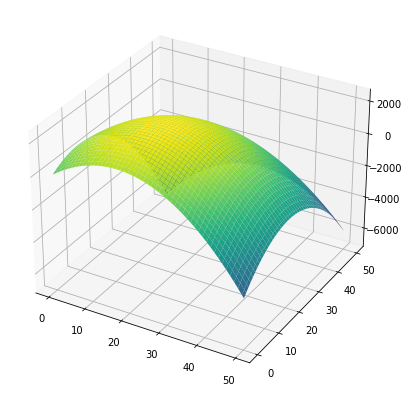
\includegraphics[width=0.5\textwidth]{images/1.png}
    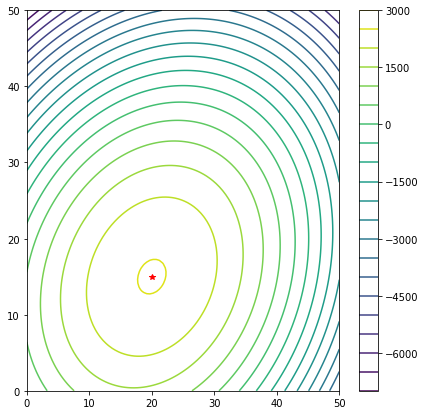
\includegraphics[width=0.5\textwidth]{images/2.png}
    \label{}
\end{figure}

\begin{flushleft}
b) trouve et affiche les extrema de la fonction bénéfice sans contrainte,à l’aide de \color{gray}{"opt.minimize"}; \end{flushleft}\\
\begin{lstlisting}
#car on ne peut pas utiliser la fonction opt.minimize 
#pour chercher le point maximum,
#donc on minimise -p qui note par "negp"
def negp(x):
    return -(v(x)-c(x))

x0 = [5,5] 
res = opt.minimize(negp,x0)
maxp = -(res.fun)
maxp
\end{lstlisting}
\begin{lstlisting}
2524.9999999999627
\end{lstlisting}

\begin{flushleft}
c) affiche les lignes de niveau, l’ensemble de contrainte(s)  \end{flushleft}\\
\begin{lstlisting}
#maillage pour le graphe
x = np.linspace(0,30,100)
y = np.linspace(0,30,100)
X,Y = np.meshgrid(x,y)
Z = p([X,Y])
#affichage de contours
fig = plt.figure(figsize=(7,7))
plt.contour(X,Y,Z,50)
plt.axis('square')
plt.plot(20,15,'r*')
plt.plot(x,-x+25,'r-')
plt.colorbar()
#affichage des contraintes
plt.fill("time", "signal", 
        data={"time": [0, 25, 0], "signal": [0, 0, 25]})
\end{lstlisting}

\begin{figure}[htb]
    \caption{les lignes de niveau, l’ensemble de contrainte(s)de p}
    \begin{center}
        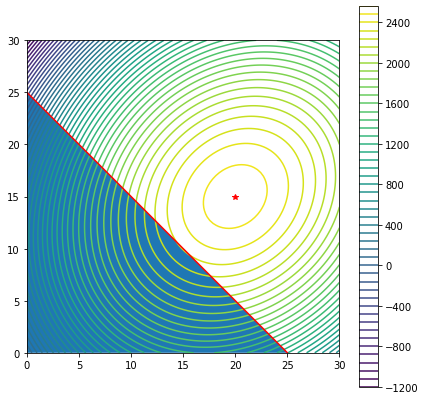
\includegraphics[width=0.35\textwidth]{images/3.png}
    \end{center}
    \label{}
\end{figure}

\begin{flushleft}
    d) trouve et affiche l'extrema sous contrainte de la fonction bénéfice.  
\end{flushleft}

\begin{lstlisting}
#gradient de p
def gradp(x):
    return [-10*x[0] -2 *x[1] + 170, -10*x[1]-2*x[0]+110]
#contrainte
cons = ({'type':  'ineq',
         'fun': lambda x: np.array(x[0]+x[1]-25)})
#meme raison que la question precedent,
#on doit minimise son negatif
negcons = ({'type':  'ineq',
         'fun': lambda x: np.array(-(x[0]+x[1]-25))})

ressc = opt.minimize(negp,x0,constraints=negcons)

maxpsc = -(ressc.fun)
maxpsc
\end{lstlisting}
\begin{lstlisting}
2324.999999999965
\end{lstlisting}

\begin{figure}[htb]
    \caption{l'extrema sous contrinte }
    \begin{center}
        \includegraphics[width=0.5\textwidth]{images/4.png}
    \end{center}
    \label{}
\end{figure}


\end{document}
